\scalebox{0.55}{
  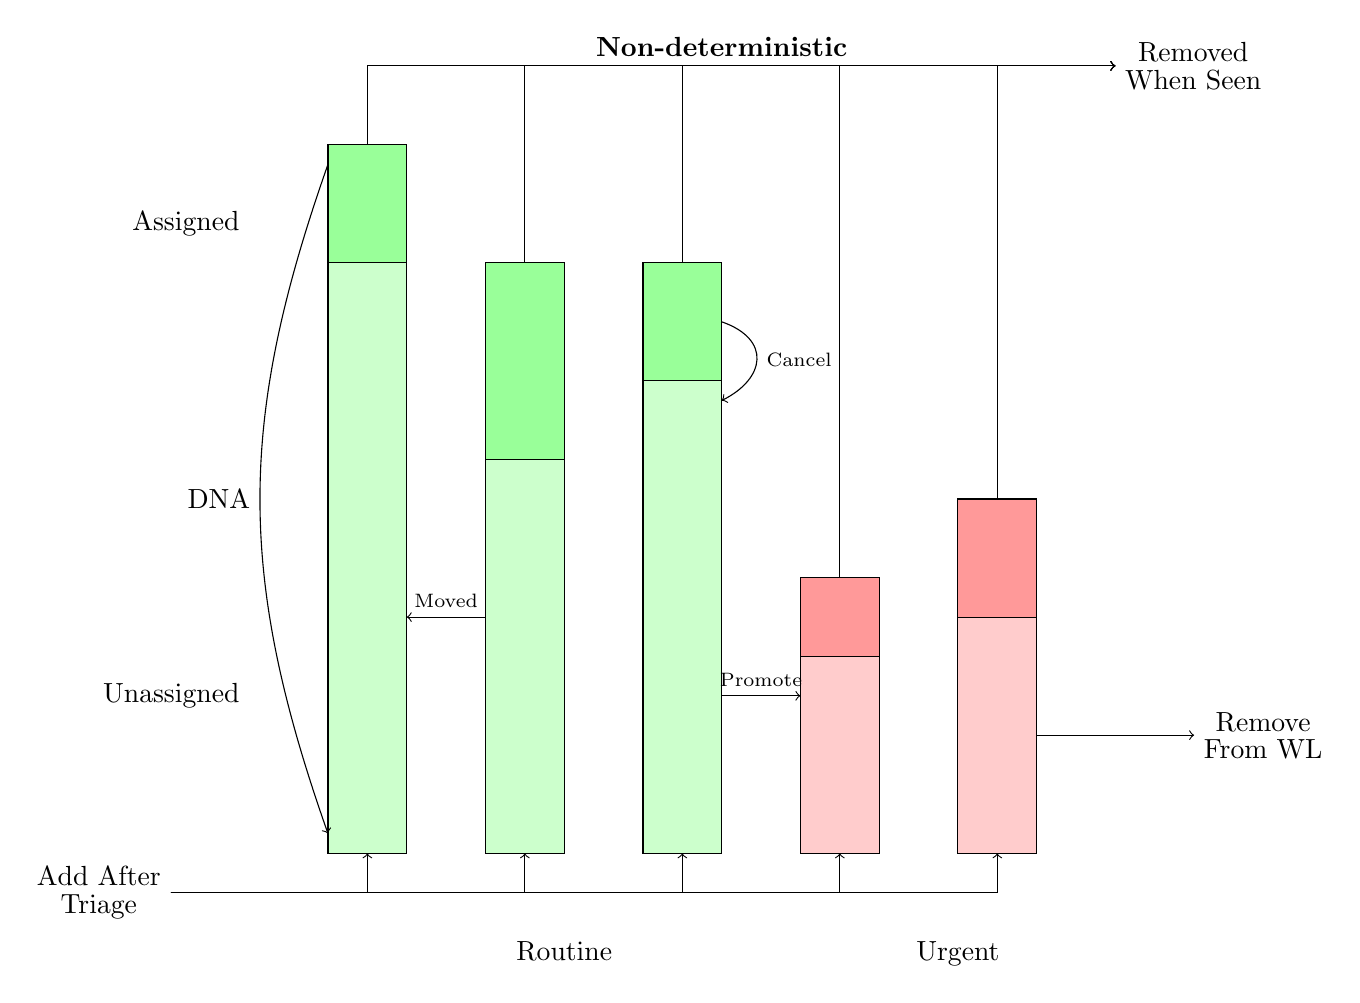
\begin{tikzpicture}[xscale=1,yscale=0.5]
  \draw[fill=green!20] (0,0) rectangle (1,15);
  \draw[fill=green!40] (0,15) rectangle (1,18);
  \draw[fill=green!20] (2,0) rectangle (3,10);
  \draw[fill=green!40] (2,10) rectangle (3,15);
  \draw[fill=green!20] (4,0) rectangle (5,12);
  \draw[fill=green!40] (4,12) rectangle (5,15);
  \draw[fill=red!20] (6,0) rectangle (7,5);
  \draw[fill=red!40] (6,5) rectangle (7,7);
  \draw[fill=red!20] (8,0) rectangle (9,6);
  \draw[fill=red!40] (8,6) rectangle (9,9);
  \node[below] at (3,-2) {Routine};
  \node[below] at (8,-2) {Urgent};
  \node[left] at (-1,4) {Unassigned};
  \node[left] at (-1,16) {Assigned};
  \draw[->] (-2,-1) -- (0.5,-1) -- (0.5,0);
  \draw[->] (-2,-1) -- (2.5,-1) -- (2.5,0);
  \draw[->] (-2,-1) -- (4.5,-1) -- (4.5,0);
  \draw[->] (-2,-1) -- (6.5,-1) -- (6.5,0);
  \draw[->] (-2,-1) -- (8.5,-1) -- (8.5,0);
  \node[left] at (-2,-1) {\shortstack{Add After\\Triage}};
  \draw[->] (0.5,18) -- (0.5,20) -- (10,20);
  \draw[->] (2.5,15) -- (2.5,20) -- (10,20);
  \draw[->] (4.5,15) -- (4.5,20) -- (10,20);
  \draw[->] (6.5,7) -- (6.5,20) -- (10,20);
  \draw[->] (8.5,9) -- (8.5,20) -- (10,20);
  \node[right] at (10,20) {\shortstack{Removed\\When Seen}};
  \node[above] at (5,20) {\textbf{Non-deterministic}};
  \draw[->] (0,17.5) to [out=260,in=100] node[left] {DNA} (0,0.5);
  \draw[->] (5,13.5) to [out=325,in=45] node[right] {\scriptsize Cancel} (5,11.5);
  \draw[->] (2,6) -- node[above] {\scriptsize Moved} (1,6);
  \draw[->] (5,4) -- node[above] {\scriptsize Promote} (6,4);
  \draw[->] (9,3) --  (11,3);
  \node[right] at (11,3) {\shortstack{Remove\\From WL}};
\end{tikzpicture}
}
